\documentclass[UTF8]{article}
\usepackage{blindtext}
\usepackage[T1]{fontenc}
\usepackage[utf8]{inputenc}
\usepackage{multirow}
\usepackage{booktabs}
\usepackage{amssymb}
\usepackage{ctex}
\usepackage{tikz}
\usepackage{listings}
\usepackage[fleqn]{amsmath}
\usepackage{xcolor}
\usepackage{color}
\usepackage{xcolor}
\usepackage{graphicx}
\usepackage{epstopdf}
\definecolor{dkgreen}{rgb}{0,0.6,0}
\definecolor{gray}{rgb}{0.5,0.5,0.5}
\definecolor{mauve}{rgb}{0.58,0,0.82}
\lstset{frame=tb,
	language=C, % 使用的语言
	aboveskip=3mm,
	belowskip=3mm,
	showstringspaces=false, % 仅在字符串中允许空格
	backgroundcolor=\color{white},   % 选择代码背景,必须加上\ usepackage {color}或\ usepackage {xcolor}
	columns=flexible,
	basicstyle = \ttfamily\small,
	numbers=none, % 给代码添加行号,可取值none, left, right.
	numberstyle=\small \color{gray},  % 行号的字号和颜色
	keywordstyle=\color{blue},
	commentstyle=\color{dkgreen}, % 设置注释格式
	stringstyle=\color{mauve},
	breaklines=true,   % 设置自动断行.
	breakatwhitespace=true, % 设置是否当且仅当在空白处自动中断.
	escapeinside=``, %逃逸字符(1左面的键),用于显示中文
	frame=single, %设置边框格式
	extendedchars=false, %解决代码跨页时,章节标题,页眉等汉字不显示的问题
	xleftmargin=0em,xrightmargin=1em, aboveskip=1em, %设置边距
	tabsize=4 % 将默认tab设置为4个空格
}
\begin{document}
	\begin{center}
	\textbf{{\huge Lab2 32位MIPS单周期处理器设计}}
	\end{center}
	\section{实验目的}
	\par 
	熟悉MIPS单周期CPU的工作原理
	
	熟悉Verilog HDL基本语法及其设计思想
	
	熟悉Vivado仿真测试的使用
	\section{实验过程}
	\begin{enumerate}
		\item [2.1] 学习MIP单周期处理器原理
		\par 首先在阅读了教材(《计算机组成与体系结构(第三版)》)的第四、五章后,对于MIPS单周期处理器的工作原理我有了更深刻的理解。对于寄存器,ALU,译码器等模块的工作原理以及共同实现的效果有了更深刻的了解。并且对如下图所示的MIPS单周期处理器的工作原理以及使用它完成各种指令时各模块的工作方式有了较全面的了解。
		\begin{figure}[htbp]
			\centering
			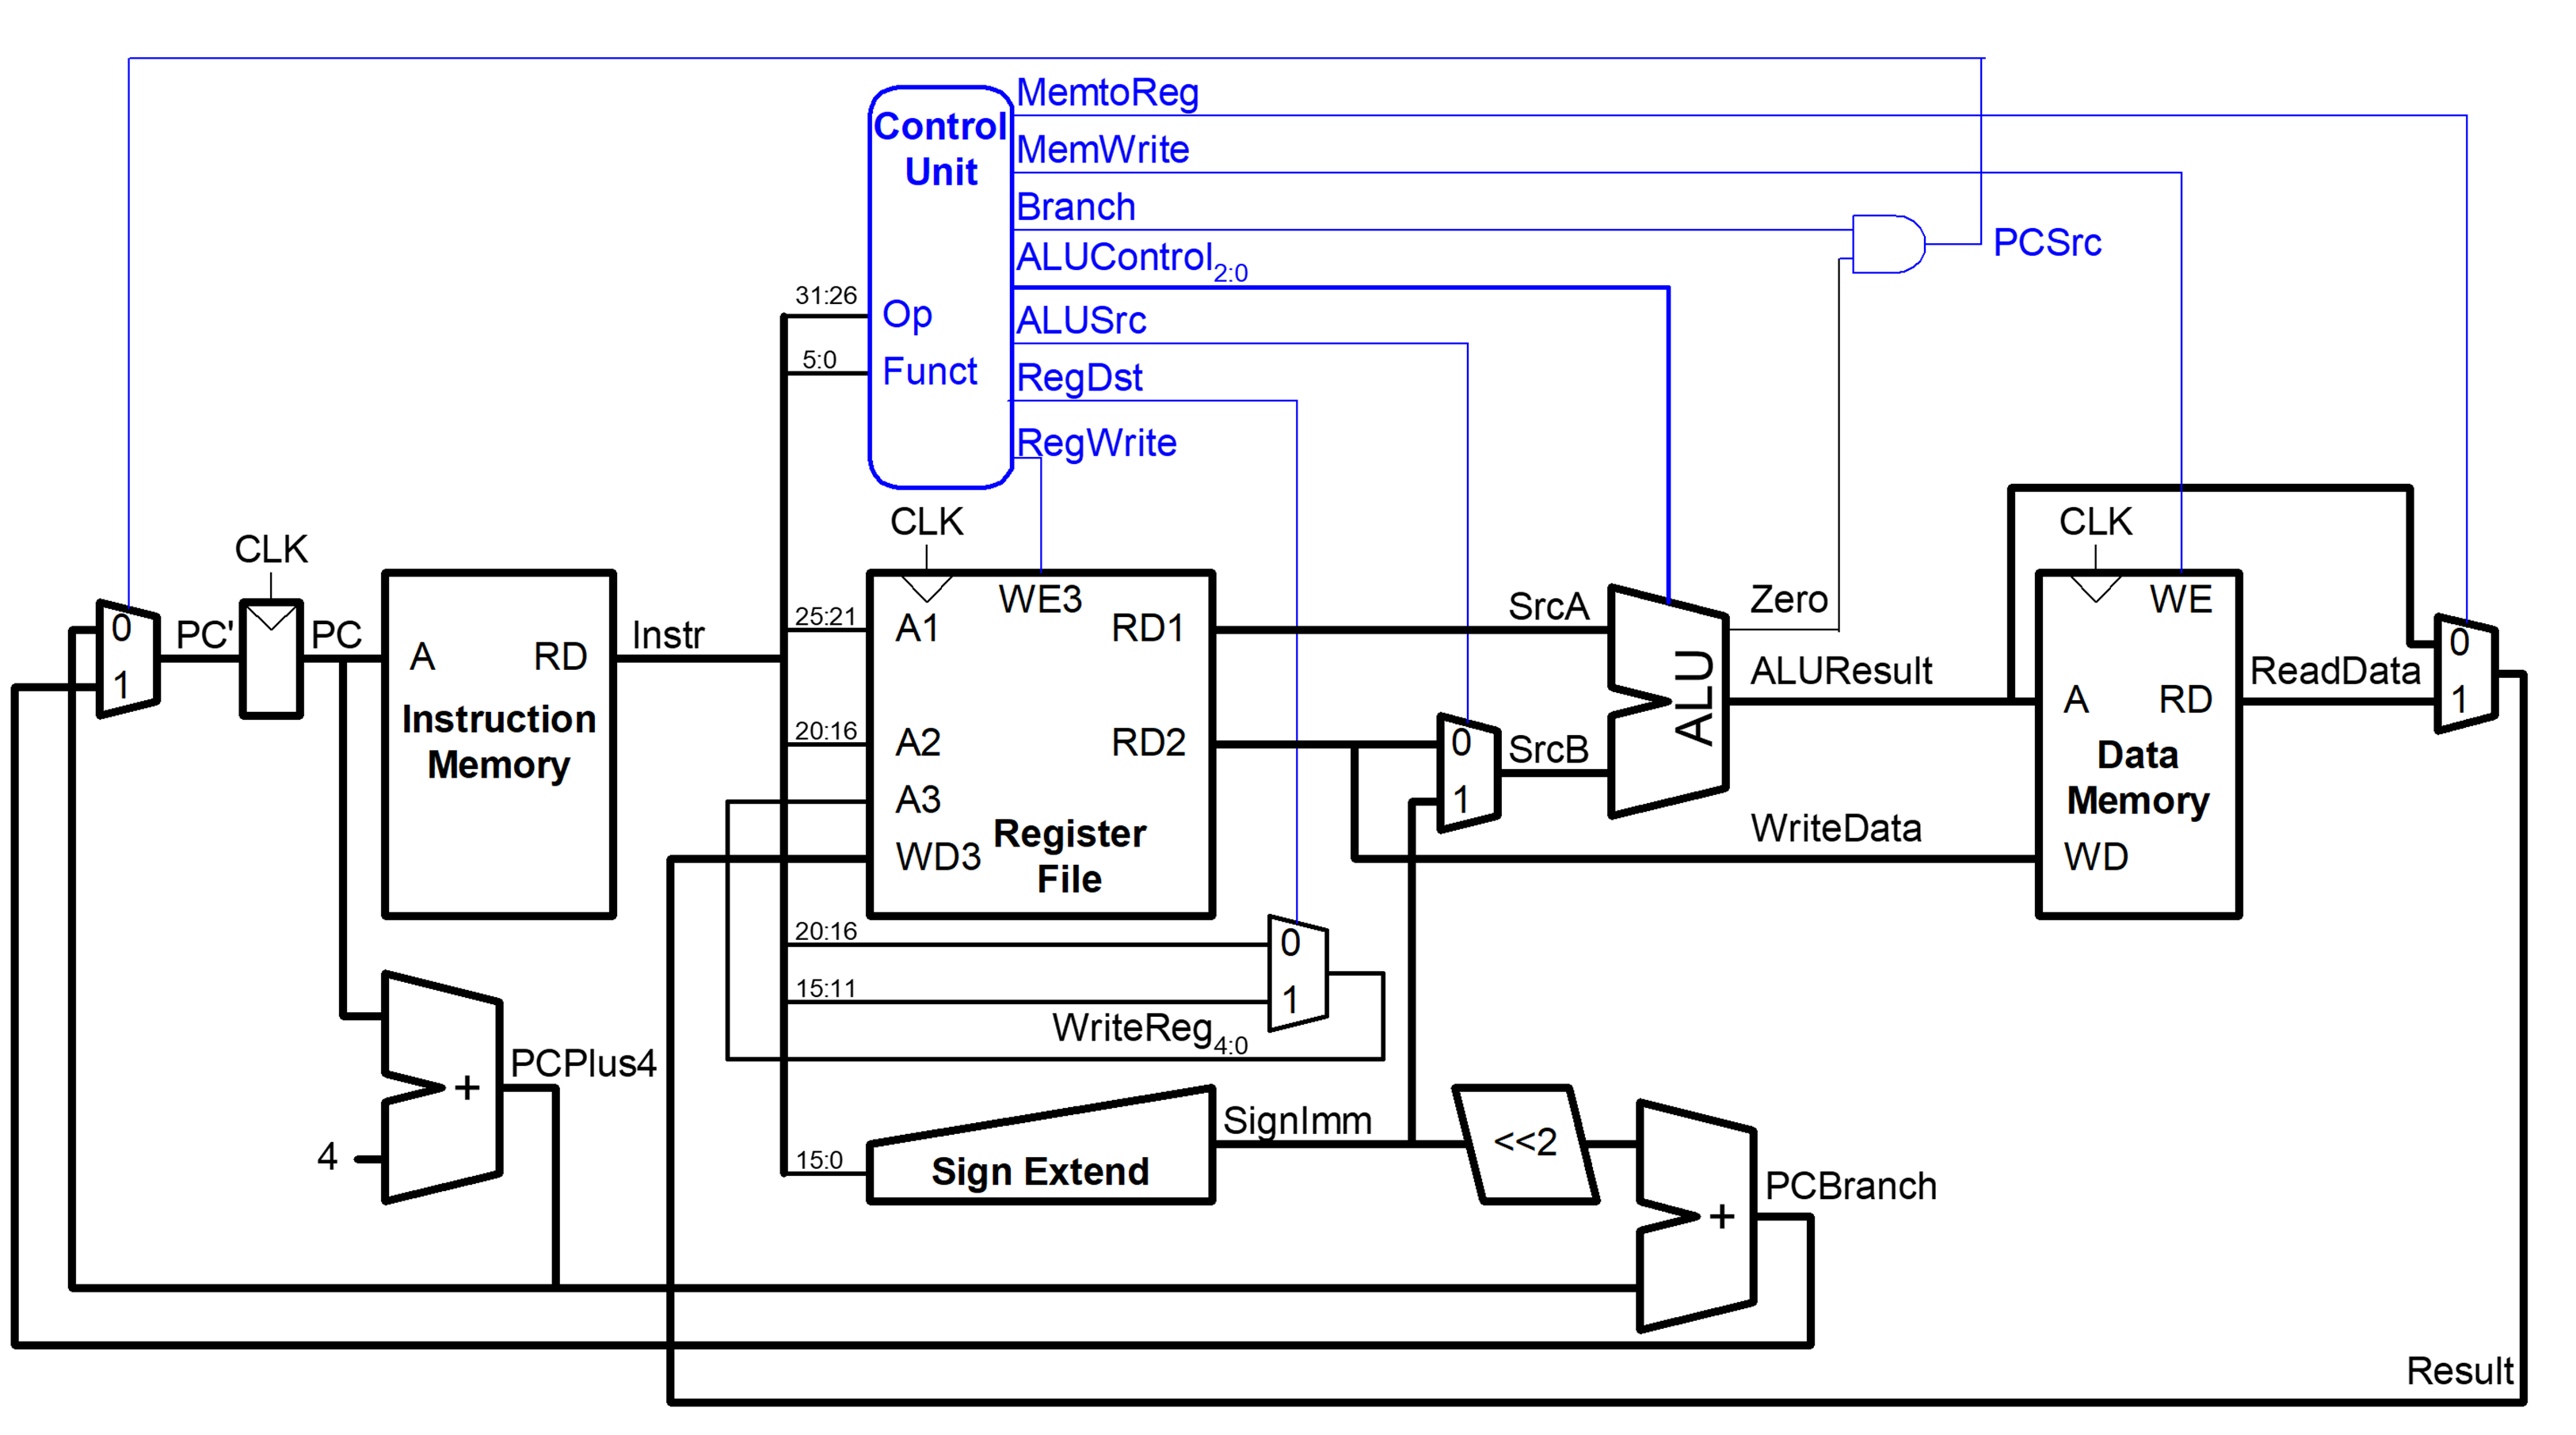
\includegraphics[scale=0.5]{2-1.png}
		\end{figure}
		\item [2.2] 完成MIPS单周期处理器设计
			\begin{enumerate}
				\item [2.2.1] 添加代码框架
					\par 根据给出的实验材料上PPT中的代码,写出代码的整体结构,如下图所示:
					\begin{figure}[htbp]
						\centering
						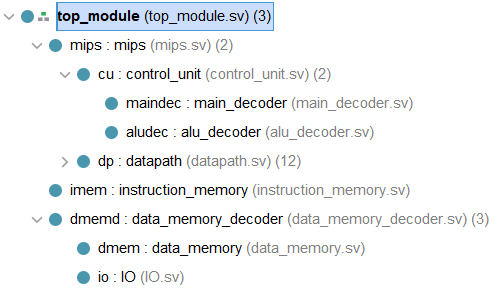
\includegraphics[scale=1]{2-2-1.png}
					\end{figure}
				\item [2.2.2] 添加指令集
					\begin{enumerate}
						\item [2.2.2.1] 指令集概览
							\par 书中只给出了一部分MIPS指令的实现方法,但可以仿照书中的方法,编写出更多MIPS指令,从而满足更多汇编代码的需求。经过编写,目前本MIP单周期处理器实现的指令集如下:\\
							\begin{tabular}{|c|c|c|} \hline
								指令 & 指令类型 & 功能         \\ \hline 
								add  & R       & 加           \\ \hline 
								sub  & R       & 减           \\ \hline 
								add  & R       & 按位与       \\ \hline 
								or   & R       & 按位或       \\ \hline 
								slt  & R       & 小于则置1    \\ \hline 
								lw   & I       & 读内存       \\ \hline 
								sw   & I       & 写内存       \\ \hline 
								addi & I       & 加立即数     \\ \hline 
								andi & I       & 按位与立即数 \\ \hline 
								ori  & I       & 按位或立即数 \\ \hline 
								beq  & I       & 相等则跳转   \\ \hline 
								j    & J       & 跳转        \\ \hline 
							\end{tabular}
						\item [2.2.2.2] 指令集实现
							\par 指令集中多数指令都已经在书中给出了其具体实现方式,这里不再赘述。一些新增的指令并不需要对处理器的结构做出大修改,只需要调整译码器和ALU,使其可以识别新的指令。
						\item [2.2.2.3] 主译码器真值表\\
							\resizebox{\textwidth}{!}{
								\begin{tabular}{|c|c|c|c|c|c|c|c|c|c|} \hline
								指令 & opcode & RegWrite & RegDst & ALUSrc & Branch & MemWrite & MemtoReg & Jump & ALUop \\ \hline 
								R类型 & 000000 & 1 & 1 & 0 & 0 & 0 & 0 & 0 & 111 \\ \hline 
								lw   & 100011 & 1 & 0 & 1 & 0 & 0 & 1 & 0 & 000 \\ \hline 
								sw   & 101011 & 0 & 0 & 1 & 0 & 1 & 0 & 0 & 000 \\ \hline 
								addi & 001000 & 1 & 0 & 1 & 0 & 0 & 0 & 0 & 000 \\ \hline 
								andi & 001100 & 1 & 0 & 1 & 0 & 0 & 0 & 0 & 011 \\ \hline 
								ori  & 001101 & 1 & 0 & 1 & 0 & 0 & 0 & 0 & 100 \\ \hline 
								beq  & 000100 & 0 & 0 & 0 & 1 & 0 & 0 & 0 & 001 \\ \hline 
								j    & 000010 & 0 & 0 & 0 & 0 & 0 & 0 & 1 & 000 \\ \hline 
							\end{tabular}}
						\item [2.2.2.4] ALUOP编码表\\
							\begin{tabular}{|c|c|} \hline
								ALUOP & 含义          \\ \hline 
								000   & 加法          \\ \hline 
								001   & 减法          \\ \hline 
								011   & 按位与        \\ \hline 
								100   & 按位或        \\ \hline 
								111   & 根据funct决定 \\ \hline 
								other & 未使用        \\ \hline 
							\end{tabular}
						\item [2.2.2.5] ALU译码器真值表\\
							\begin{tabular}{|c|c|c|} \hline
								ALUop & Funct  & ALUControl\\ \hline 
								000   & x      & 加        \\ \hline 
								001   & x      & 减        \\ \hline 
								011   & x      & 按位与    \\ \hline 
								100   & x      & 按位或    \\ \hline 
								111   & 100000 & 加        \\ \hline 
								111   & 100010 & 减        \\ \hline 
								111   & 100100 & 按位与    \\ \hline 
								111   & 100101 & 按位或    \\ \hline 
								111   & 101010 & 小于则置1 \\ \hline 
								other & x      & 未使用    \\ \hline 
							\end{tabular}
					\end{enumerate}
			\end{enumerate}
		\item [2.3] 测试代码
			\par 为了便于测试,本CPU还实现了IO接口,可通过开关实时控制CPU中运算的数值。原理为在内存中高位设置一块接口区,其中包含两个操作数的值、一个结果的值和一个状态数,当访问到内存中的高位时,改为从接口区读取数值,同时在代码中通过判断状态数决定是否进行跳转,从而使输入可以即时反映到代码。具体则是通过扩展DataMemory实现。最后添加和7段数码管的衔接,从而将结果显示出来。结构图如下图所示:
			\begin{figure}[htbp]
				\centering
				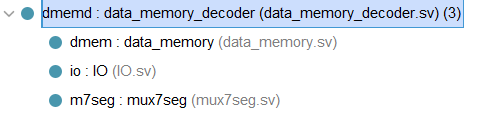
\includegraphics[scale=1]{2-3.png}
			\end{figure}
			$data_memory_decoder:$将下列三个模块衔接起来;
			
			$data_memory:$修改前的DataMemory,扩展了内存用来进行IO接口;
			
			$IO:$判断状态数,存储三个数的数值,并将数值传输给下一个模块;
			
			$mux7seg:$用7段数码管显示三个数;
			
			\par 接下来先进行实验材料中PPT上的MIPS测试代码的仿真,测试结果如下图:
			\begin{figure}[htbp]
				\centering
				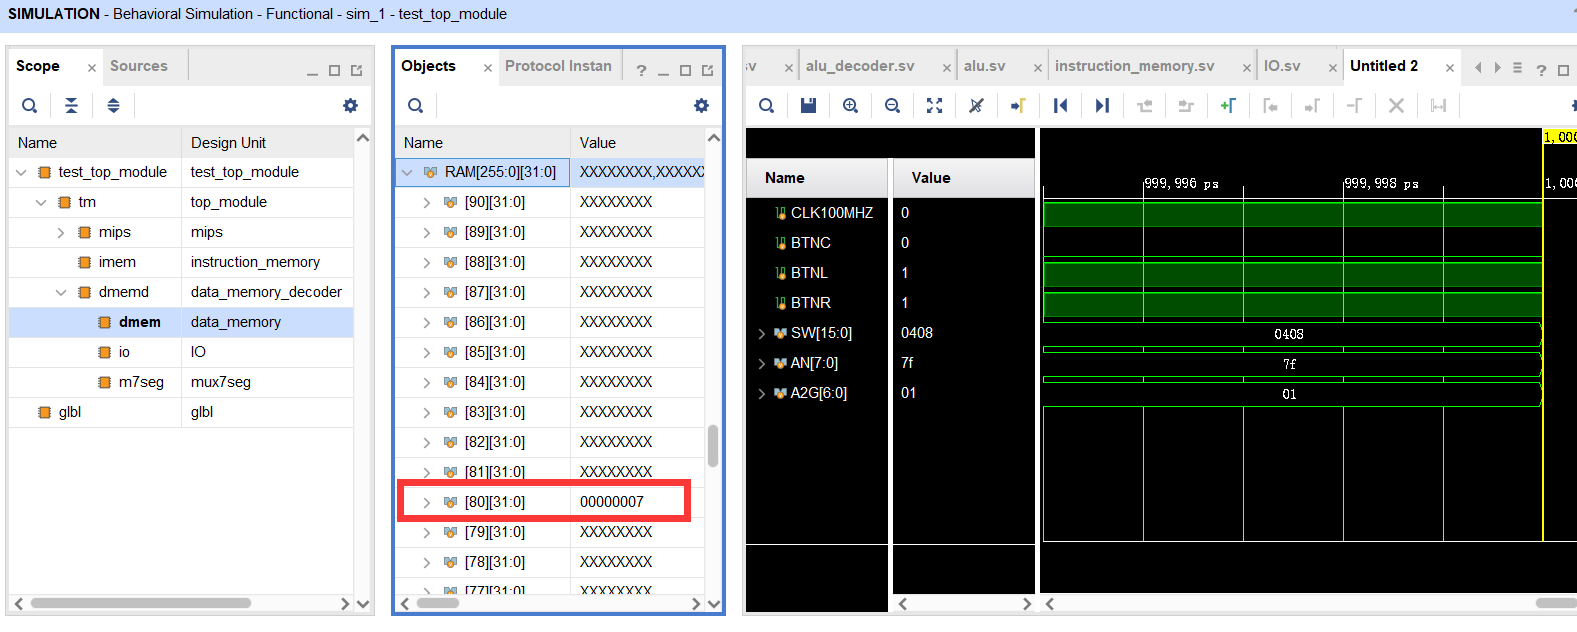
\includegraphics[scale=0.4]{2-3-1.png}
			\end{figure}
			\par 可以看到在运行结束后内存中的80位存入了7,与代码设计相符。
			
			\par 然后进行关于IO接口的MIPS测试代码的仿真,其中IO接口的MIPS测试代码如下:
			\begin{figure}[htbp]
				\centering
				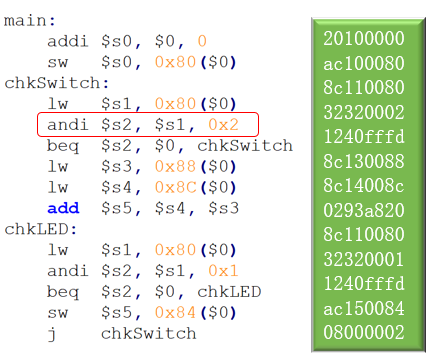
\includegraphics[scale=1]{2-3-2.png}
			\end{figure}
			\par 测试结果如下图:
			\begin{figure}[htbp]
				\centering
				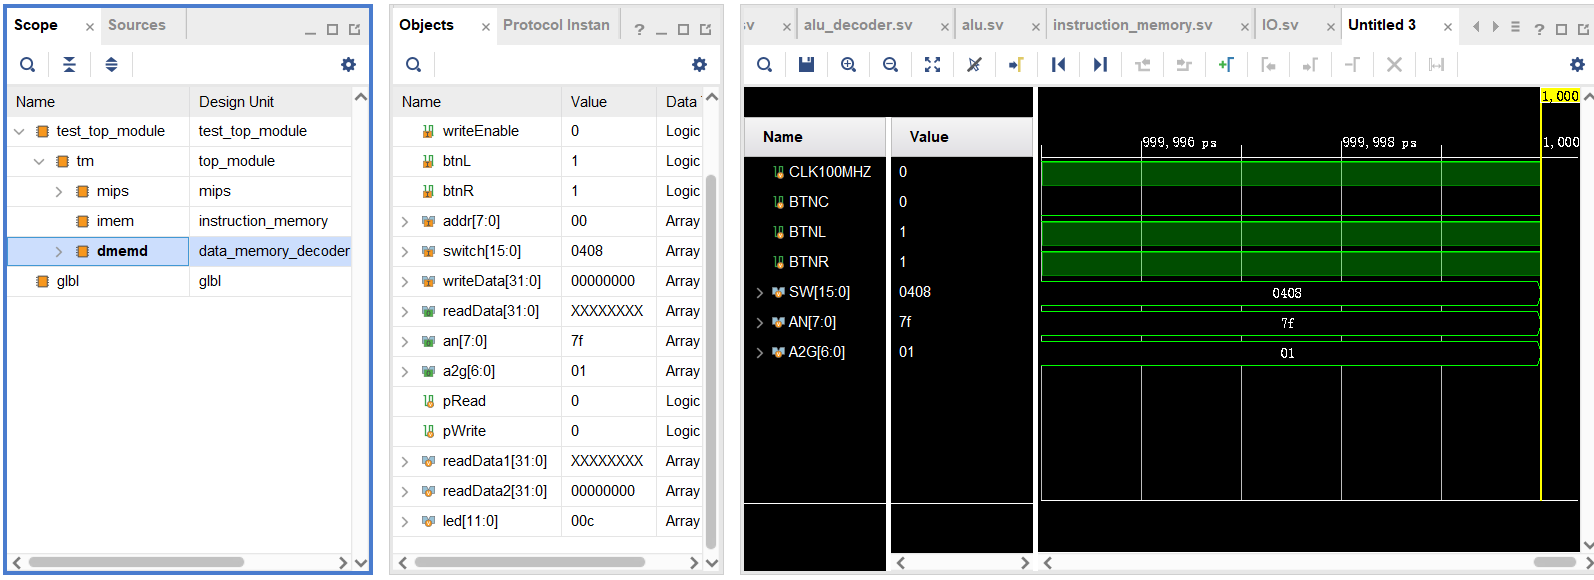
\includegraphics[scale=0.4]{2-3-3.png}
			\end{figure}
			\par 可以看到在运行结束后led变量存入了0000000c,即十进制的12,与代码中应存入的4+8的结果相符。
			
			\par 最后进行实机测试,测试结果如下图:
			\begin{figure}[htbp]
				\centering
				\includegraphics[scale=0.2]{2-3-4.jpg}
			\end{figure}
	\end{enumerate}
	\section{实现体会}
	\par 在本次实验过程中我有很多的收获。首先在阅读教材之后,使我更加熟悉了MIPS单周期处理器的寄存器,加法器,左移单位,符号扩展单元,alu,可复位触发器和复用器等模块的工作原理以及其在MIPS处理器设计时的代码设计思路。在使用vivado的过程中,我学习到了软件的相关操作,主要是对项目以及模块的创建过程以及仿真测试,上板测试的操作过程,尤其是使用仿真对代码进行调试,使用下来发现非常方便,令我受益匪浅。
\end{document}